
%%%%%%%%%%%%%%%%% Intro %%%
\section{Introduction}
In this report various methods for the estimation of parameters of a given data set are evaluated and compared. To cut down the problem's complexity, we use a simple model for the flux of an elliptic galaxy, as is described by the Sersic profile, which provides us an initial data set. This data set - a noisy image of a elliptic galaxy as it would have been taken by a ground-based telescope - is then used to evaluate different estimation approaches as the least square estimation, maximum likelihood estimation and Bayesian estimation.\\
%Specifically, with these estimators the parameters for the flux of a galaxy is

\section{Modelling a galaxy}
The Sersic profile is very common amongst astrophysicists to model the flux of observed elliptic galaxies in a simple way, and is given by the equation

\begin{equation}
	\centering
	I(l,c) = exp(-R(l,c)^{\frac{1}{n}})
\end{equation}

which describes the variation of intensity with respect to the distance of the galaxy's centre.
The distance $R$ of a pixel with the coordinates $(l,c)$ from the galaxies centre is given by 

\begin{equation}
	\centering
	R(l,c)^2 = \bigg(\frac{(l-l_0)\sin(\alpha) - (c - c_0)\cos(\alpha)}{\sigma_l}\bigg)^2 + \bigg(\frac{(l-l_0)\cos(\alpha) - (c - c_0)\sin(\alpha)}{\sigma_c}\bigg)^2
\end{equation}

with $(l_0,c_0)$ being the galaxy's centre coordinates, $(\sigma_l,\sigma_c)$ the two galaxy's axes length and the horizontal angle $\alpha$.

This leads to the following equation modelling the data

\begin{equation}
	\centering
	d(l,c) = s + a I(l,c) + n(l,c)
\label{eq:dlc}
\end{equation}

with $a$ as the amplitude of the galaxy, $s$ the amplitude of the sky's background and $n(l,c)$ as noise.


Using the Sersic profile we can now generate an artificial elliptic galaxy, see \cref{fig:initial}.


\begin{figure}[!h]
	\centering
	\begin{minipage}[b]{0.4\textwidth}
		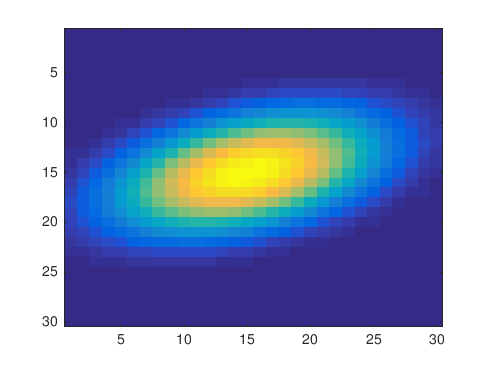
\includegraphics[width=\textwidth]{images/galaxy_initial}
		\caption{Initial data set}
		\label{fig:initial}
	\end{minipage}
	\begin{minipage}[b]{0.4\textwidth}
		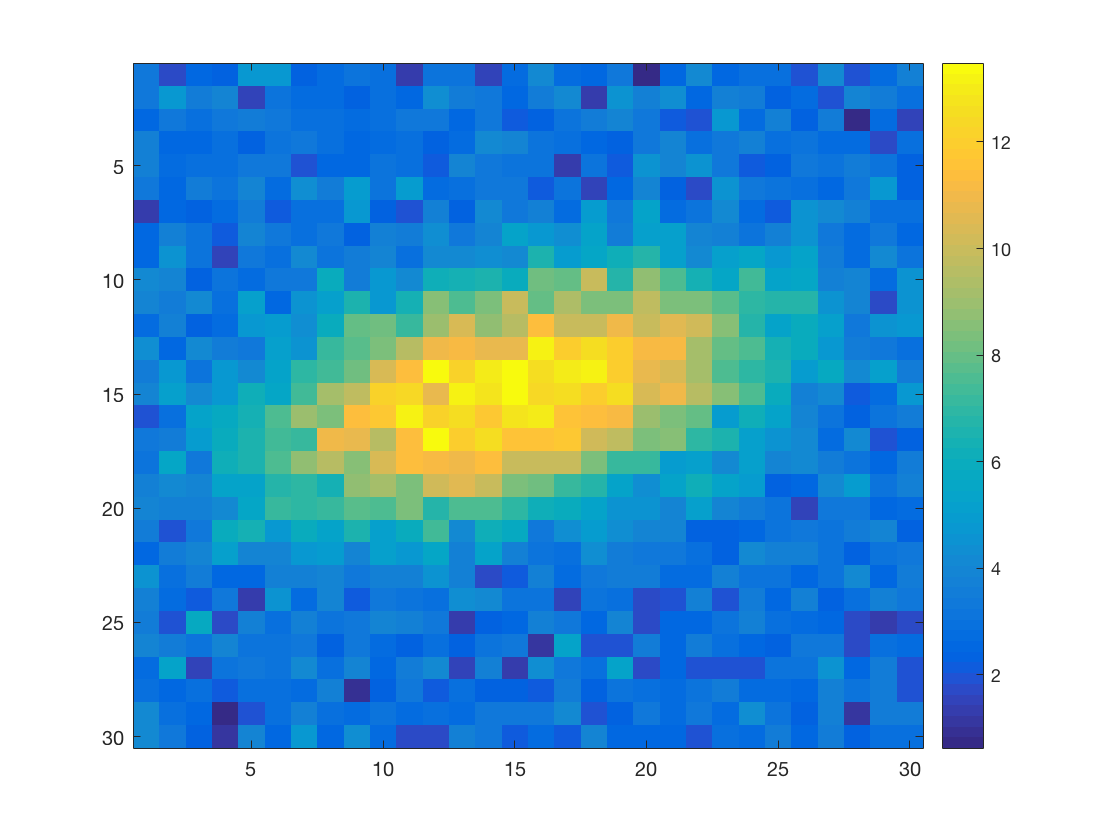
\includegraphics[width=\textwidth]{images/galaxy_noise}
		\caption{Random noise added}
		\label{fig:addedNoise}
	\end{minipage}
\end{figure}

By assuming a Gaussian white noise with the known variance $\sigma_n^2$ and using the initial image of the galaxy, we can model the elliptic galaxy as it would have been seen by a ground-based telescope, see \cref{fig:addedNoise}.



The parameters used to create above mentioned figure are given as follows


	\begin{align*}
		L, C & = 30px & l_0, c_0 & = 15 & \sigma_l & = 10 & \sigma_c & = 5 \\
		\alpha & = 0.3 & n & = 0.4 & a & = 10 & s & = 3 
	\end{align*}

with $L,C$ as height respectively width of image in pixels, $l_0, c_0$ the galaxy's centre in pixel coordinates and $\sigma_l, \sigma_c$ as length parameters.
\todo{probalby don't need this explananation here, see above text}





%%%%%%%%%%%%%%%%% TASK 1 %%%
\section{Estimation with known Galaxy's location and shape parameters}
Having successfully modelled a simple elliptic galaxy, this model is used as input data for the simulation of an estimation of the galaxy's and sky background's amplitude, while assuming that the galaxy's position and shape parameters are known. This estimation can be formulated via:
\begin{equation}
\boldsymbol{y}=\boldsymbol{H}\boldsymbol{\theta}+\boldsymbol{n}(c,l)
\label{eq:generalestimation}
\end{equation}
Here, $\boldsymbol{y}$ is the actual measurement, in our case it is the intensity of the galaxy. However, one has to keep in mind that for the  following steps, we use the simulated galaxy intensity as described above as our measured galaxy intensity. $\boldsymbol{\theta}$ is the vector of estimated parameters, which are in our case the galaxy's amplitude $a$ and the background's amplitude $s$, so $\boldsymbol{\theta}=[s,a]^{\mathrm{T}}$. $\boldsymbol{H}$ is a matrix describing the underlying model, which in our case also depends on the pixel position since the intensity described by the sersic function depends on the distance towards the centre of the galaxy, and $\boldsymbol{n}(l,c)$ is a noise component also depending on the pixel position (l,c). In order to satisfy equation \ref{eq:dlc} using equation \ref{eq:generalestimation}, one has to define $\boldsymbol{H}$ in a special matrix form, which is given by:
\begin{equation}
H_{l,c}=\left(\begin{array}{cc}1& \exp(-R_{l,c}^{\frac{1}{n}}) \end{array}\right)\\
\end{equation}
Thus, $\boldsymbol{H}$ is a $2\times (L\cdot C)$ matrix, describing the intensity profile of the galaxy for each pixel (l,c). Therefore, our data $\boldsymbol{d}$ describing the measured data for all pixels yields:
\begin{equation}
\boldsymbol{d}=\boldsymbol{H}\boldsymbol{\theta}+\boldsymbol{n}(c,l),
\label{eq:generalestimation}
\end{equation}
where $d$ is a vector with $L\cdot C$ elements.\\
\newline
In order the obtain maximum likelihood estimator for $\boldsymbol{\theta}$ as a function of $\boldsymbol{d}$, one has to calculate:
\begin{equation}
\boldsymbol{\theta}=\left(\boldsymbol{H'H}\right)^{-1}\cdot\boldsymbol{H}\cdot\boldsymbol{d}
\end{equation}
The bias of that estimator could be calculated using $b_{\boldsymbol{\theta}}(\boldsymbol{\theta}_{init})=E_{Y|\boldsymbol{\theta}_{init}}(\boldsymbol{\theta})-\boldsymbol{\theta}_{init}$, where $\boldsymbol{\theta}_{init}$ is the vector of the true parameters that we want to find out. However, this bias is only applicable for a larger sets of simulations.
The used matlab code performing this is shown in the appendix. The resulting maximum likelihood estimators for the galaxy's and the sky background's amplitudes are:
\begin{equation*}
\boldsymbol{\theta}=\left[2.9576\;10.0131 \right]^{\mathrm{T}}
\end{equation*}
This result is very close to the original parameters used for the simulation of the data with $ \boldsymbol{\theta}_{initial}=\left[3\;10 \right]^{\mathrm{T}}$ (see list of parameters above). However, we assumed the galaxy center and shape to be known, which drastically reduces the number of unknowns in this fit, and therefore results in a very good fit result.

%%%%%%%%%%%%%%%%% TASK 2 %%%
\section{Maximum likelihood estimation of all parameters}
In the next step, we assumed that the galaxy's position and shape are unknown for the fit. Thus, now also the parameter vector $\boldsymbol{\nu}=\left[l_{0},c_{0}, \sigma_{l}, \sigma_{c},n\right]$ also needs to be fitted simultaniously to $\theta$. Again, the corresponding model can be formulated as:
\begin{equation*}
\boldsymbol{d}=\boldsymbol{H}(\boldsymbol{\nu})\boldsymbol{\theta}+\boldsymbol{n}(c,l),
\end{equation*}
The only difference now is that $\boldsymbol{H}$ depends on the variable $\boldsymbol{\nu}$. Again, $\boldsymbol{H}$ is a $2\times(\L\cdot C)$ - matrix, $\theta=\left[s,a\right]^{\mathrm{T}}$, $\boldsymbol{d}$ a vector with $L\cdot C$ components and $\$\boldsymbol{\nu}$ as defined above a vector with six components. The goal is to obtain the maximum likelihood estimator by minimizing the quadratic cost function $\boldsymbol{J}$:

\begin{equation}
\boldsymbol{J}(\boldsymbol{\theta,\nu})=\left(\boldsymbol{d}-\boldsymbol{H}(\boldsymbol{\nu})\boldsymbol{\theta}\right)^{\mathrm{T}}\left(\boldsymbol{d}-\boldsymbol{H}(\boldsymbol{\nu})\boldsymbol{\theta}\right)
\label{eq:costfunction}
\end{equation}
The optimization problem thus is a least square optimization. The maximum likelihood estimators are then given by:
\begin{equation*}
\left(\boldsymbol{\theta}_{ML},\boldsymbol{\nu}_{ML}\right)=argmin\left(\boldsymbol{J}\right)
\end{equation*}

For a large number of samples, this maximum likelihood estimator is unbiased with a variance equal to the inverse of the Fisher matrix: $\boldsymbol{\sigma}^{2}=\boldsymbol{F}(\boldsymbol{\theta})^{-1}$

%%%%%% arty part form here

\begin{figure}[h!]
	\centering
	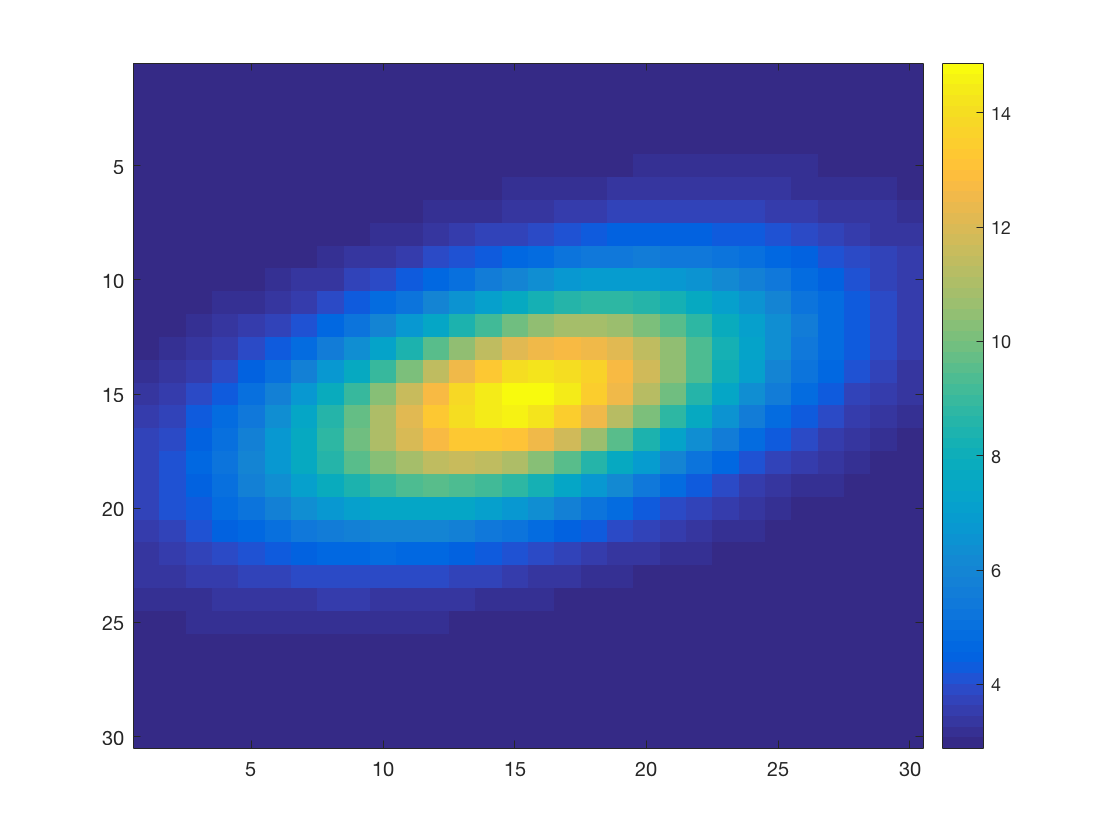
\includegraphics[width=\textwidth/2]{images/galaxy_MLE}
	\caption{estimated galaxy from noisy data}
	\label{fig:MLE}
\end{figure}

%parameters for that image:    
%3.0127
%   10.2206
%   14.9382
%   15.1359
%    4.8007
%    9.7990
%   -1.2578
%    0.4017


%%%%%%%%%%%%%%%%% TASK 3 %%%
\section{Estimation in the Bayesian framework}

\subsection{Maximum a posteriori estimator}

\subsection{Posterior mean estimator}


